\PassOptionsToPackage{table}{xcolor}
\documentclass[aspectratio=169,12pt]{beamer}
\usepackage[T1]{fontenc}
\usepackage{lmodern}
\usepackage{tikz}
\usetikzlibrary{arrows.meta,positioning,fit,backgrounds,decorations.pathreplacing}
\usepackage{xcolor}
\usepackage{array}
\usepackage{mdframed}
\usepackage{listings}
\lstset{
  basicstyle=\ttfamily\small,
  keywordstyle=\color{Navy}\bfseries,
  commentstyle=\color{MidGray}\itshape,
  backgroundcolor=\color{NavyDk!6},
  frame=single, framerule=0pt,
  xleftmargin=6pt, xrightmargin=6pt,
  aboveskip=4pt, belowskip=2pt,
  language=C
}

%% ── Colours ──────────────────────────────────────────────────
\definecolor{NavyDk}{HTML}{0D1B2A}
\definecolor{Navy}{HTML}{1B3A6B}
\definecolor{Teal}{HTML}{0A7C7B}
\definecolor{Orange}{HTML}{E8921A}
\definecolor{SlideGray}{HTML}{EEF3F8}
\definecolor{MidGray}{HTML}{5A6070}
\definecolor{LtGray}{HTML}{C0C8D8}
\definecolor{BoxGray}{HTML}{5A6880}
\definecolor{GreenHi}{HTML}{2A7A3A}

%% ── Beamer setup ─────────────────────────────────────────────
\usetheme{default}
\setbeamersize{text margin left=0.8cm,text margin right=0.8cm}
\setbeamertemplate{navigation symbols}{}

%% Background for content slides
\setbeamercolor{background canvas}{bg=SlideGray}

%% Frametitle
\setbeamercolor{frametitle}{fg=Navy,bg=SlideGray}
\setbeamerfont{frametitle}{size=\large,series=\bfseries}
\setbeamertemplate{frametitle}{%
  \vspace{0.25cm}%
  {\usebeamerfont{frametitle}\usebeamercolor[fg]{frametitle}\insertframetitle}\\[-4pt]%
  {\color{Orange}\rule{\textwidth}{2.5pt}}%
}

%% Footline
\setbeamertemplate{footline}{%
  \vspace{2pt}%
  \hspace{0.6cm}{\color{MidGray}\fontsize{7.5}{9}\selectfont
    Hardware / Software Codesign \enspace|\enspace 2025/26 \enspace|\enspace IST}%
  \hfill%
  {\color{MidGray}\fontsize{7.5}{9}\selectfont\insertframenumber}%
  \hspace{0.5cm}\vspace{3pt}%
}

\begin{document}

%% ══════════════════════════════════════════════════════════
%%  SLIDE 1 — Title
%% ══════════════════════════════════════════════════════════
{
\setbeamercolor{background canvas}{bg=NavyDk}
\setbeamertemplate{footline}{%
  \vspace{2pt}%
  \hspace{0.6cm}{\color{LtGray}\fontsize{7.5}{9}\selectfont
    Hardware / Software Codesign \enspace|\enspace 2025/26 \enspace|\enspace IST}%
  \hfill%
  {\color{LtGray}\fontsize{7.5}{9}\selectfont\insertframenumber}%
  \hspace{0.5cm}\vspace{3pt}%
}
\begin{frame}[plain]
  \vspace{0.6cm}
  \begin{center}
    {\color{white}\fontsize{32}{38}\selectfont\textbf{HLS Optimisation}}\\[0.15cm]
    {\color{Orange}\fontsize{22}{26}\selectfont\textbf{\& Float / Fixed Intro}}\\[0.4cm]
    {\color{LtGray}\fontsize{11}{14}\selectfont
      L6 \enspace$\cdot$\enspace Week 3 \enspace$\cdot$\enspace Hardware / Software Codesign 2025/26}\\[0.1cm]
    {\color{LtGray}\fontsize{10}{12}\selectfont José T.\ de Sousa \enspace$\cdot$\enspace IST}
  \end{center}
  \vspace{0.5cm}
  \begin{center}
  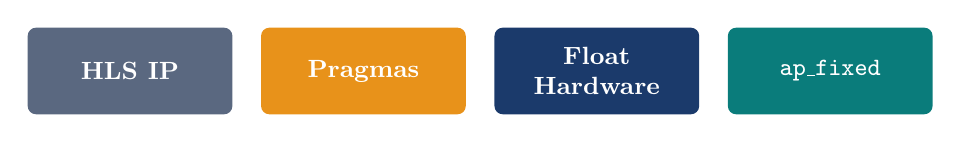
\begin{tikzpicture}[
    box/.style={rounded corners=3pt, minimum width=2.6cm, minimum height=1.1cm,
                align=center, font=\small\bfseries},
    node distance=0.35cm
  ]
    \node[box, fill=BoxGray,    text=white] (ip)   {HLS IP};
    \node[box, fill=Orange,     text=white, right=of ip]  (pp)   {Pragmas};
    \node[box, fill=Navy,       text=white, right=of pp]  (fl)   {Float\\Hardware};
    \node[box, fill=Teal,       text=white, right=of fl]  (fx)   {\texttt{ap\_fixed}};
  \end{tikzpicture}
  \end{center}
  \vspace{0.3cm}
  \begin{center}
    {\color{LtGray}\itshape\fontsize{10}{12}\selectfont
      Making your IP faster — and understanding what data types cost in silicon}
  \end{center}
\end{frame}
}

%% ══════════════════════════════════════════════════════════
%%  SLIDE 2 — Where We Are
%% ══════════════════════════════════════════════════════════
\begin{frame}{Where We Are}
\vspace{0.1cm}
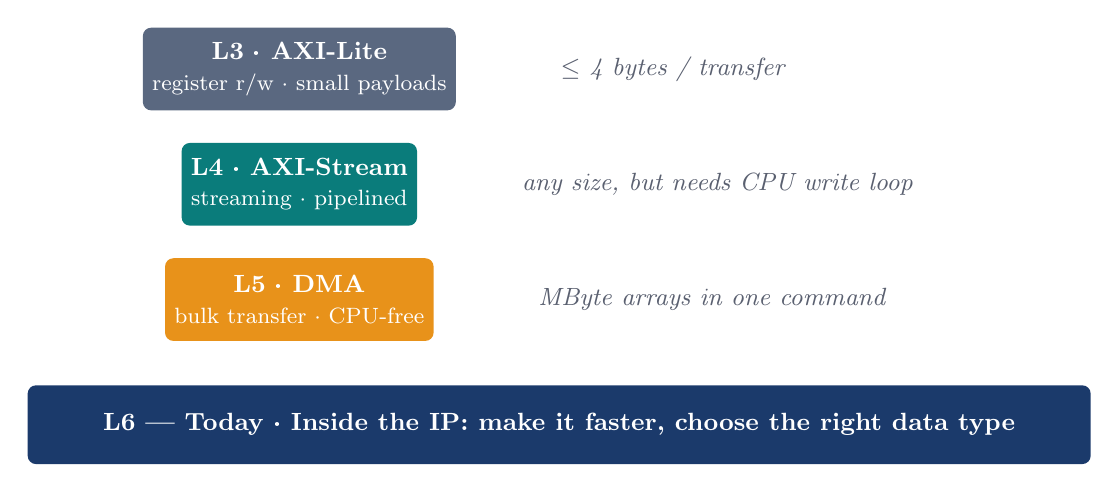
\begin{tikzpicture}[
  lbl/.style={rounded corners=3pt, minimum width=2.4cm, minimum height=1.05cm,
              align=center, font=\small\bfseries, text=white},
  note/.style={align=left, font=\small\itshape, text=MidGray},
  node distance=0.4cm
]
  %% Lecture boxes (stacked left)
  \node[lbl, fill=BoxGray]  (l3) {\textbf{L3} \textperiodcentered\ AXI-Lite\\{\normalfont\fontsize{8}{10}\selectfont register r/w $\cdot$ small payloads}};
  \node[lbl, fill=Teal,     below=of l3] (l4) {\textbf{L4} \textperiodcentered\ AXI-Stream\\{\normalfont\fontsize{8}{10}\selectfont streaming $\cdot$ pipelined}};
  \node[lbl, fill=Orange,   below=of l4] (l5) {\textbf{L5} \textperiodcentered\ DMA\\{\normalfont\fontsize{8}{10}\selectfont bulk transfer $\cdot$ CPU-free}};

  %% Notes to the right of each box
  \node[note, right=1.2cm of l3] {$\leq$ 4 bytes / transfer};
  \node[note, right=1.2cm of l4] {any size, but needs CPU write loop};
  \node[note, right=1.2cm of l5] {MByte arrays in one command};

  %% L6 highlight box — full width
  \node[lbl, fill=Navy, minimum width=13.5cm, minimum height=1.0cm,
        below=0.55cm of l5, xshift=3.3cm]
    (l6) {\textbf{L6 — Today} \textperiodcentered\ Inside the IP: make it faster, choose the right data type};
\end{tikzpicture}

\vspace{0.3cm}
{\color{Teal}\itshape\small The interface chain is complete.
  Today we zoom inside the IP and ask: how fast can it go, and what does float actually cost?}
\end{frame}

%% ══════════════════════════════════════════════════════════
%%  SLIDE 3 — Today's Two Questions
%% ══════════════════════════════════════════════════════════
\begin{frame}[t]{Today's Two Questions}
\vspace{0.15cm}
\begin{columns}[T,totalwidth=\textwidth]

  \column{0.49\textwidth}
  \colorbox{Orange!10}{\parbox{\dimexpr\linewidth-2\fboxsep\relax}{%
    \vspace{3pt}
    {\color{Orange}\bfseries (1) Can we make the IP faster?}\\[3pt]
    {\small Run faster without changing what it computes?}\\[4pt]
    {\small\color{Navy}
    \begin{itemize}\setlength{\itemsep}{1pt}
      \item Initiation Interval (II) — limits throughput
      \item \texttt{PIPELINE}, \texttt{UNROLL}, \texttt{ARRAY\_PARTITION}
      \item Reading the HLS synthesis report
    \end{itemize}}
    \vspace{2pt}
    {\small\itshape\color{MidGray}Goal: II\,=\,1 on the inner loop.}
    \vspace{3pt}
  }}

  \column{0.02\textwidth}

  \column{0.49\textwidth}
  \colorbox{Teal!10}{\parbox{\dimexpr\linewidth-2\fboxsep\relax}{%
    \vspace{3pt}
    {\color{Teal}\bfseries (2) What does \texttt{float} cost in HW?}\\[3pt]
    {\small A float adder is a multi-stage pipeline: $\sim$400\,LUTs, not a single gate.}\\[4pt]
    {\small\color{Navy}
    \begin{itemize}\setlength{\itemsep}{1pt}
      \item Why the FP accumulator gets II\,=\,4
      \item \texttt{ap\_fixed<W,I>} as the fix
      \item Area vs.\ accuracy trade-off (L7 preview)
    \end{itemize}}
    \vspace{2pt}
    {\small\itshape\color{MidGray}Goal: know the cost before choosing a type.}
    \vspace{3pt}
  }}

\end{columns}
\end{frame}


%% ══════════════════════════════════════════════════════════
%%  SECTION 2 — HLS PERFORMANCE MODEL
%% ══════════════════════════════════════════════════════════

%% ── SLIDE 4 : Latency vs Throughput — the II concept ──────
\begin{frame}{Latency vs.\ Throughput: What Is II?}
\vspace{0.1cm}
\begin{columns}[T,totalwidth=\textwidth]

  \column{0.55\textwidth}
  \vspace{0.1cm}
  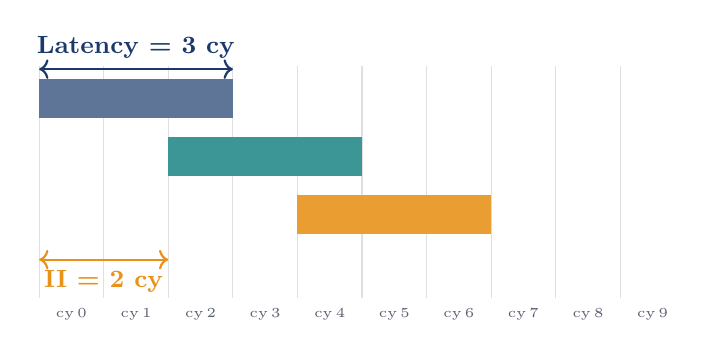
\begin{tikzpicture}[scale=0.82]
    % Grid background
    \foreach \x in {0,...,9} \draw[gray!25,thin] (\x,0) -- (\x,3.6);
    % Cycle labels
    \foreach \x/\l in {0/0,1/1,2/2,3/3,4/4,5/5,6/6,7/7,8/8,9/9}
      \node[font=\tiny\color{MidGray}] at (\x+0.5,-0.25) {cy\,\l};
    % Iteration 0
    \fill[Navy!70]   (0,2.8) rectangle (3,3.4) node[midway,font=\tiny\bfseries\color{white}]{iter 0};
    % Iteration 1 (starts at II=2)
    \fill[Teal!80]   (2,1.9) rectangle (5,2.5) node[midway,font=\tiny\bfseries\color{white}]{iter 1};
    % Iteration 2
    \fill[Orange!90] (4,1.0) rectangle (7,1.6) node[midway,font=\tiny\bfseries\color{white}]{iter 2};
    % Latency brace for iter 0
    \draw[<->,thick,Navy] (0,3.55) -- (3,3.55) node[midway,above,font=\small\color{Navy}]{\textbf{Latency = 3 cy}};
    % II brace
    \draw[<->,thick,Orange] (0,0.6) -- (2,0.6) node[midway,below,font=\small\color{Orange}]{\textbf{II = 2 cy}};
  \end{tikzpicture}

  \column{0.45\textwidth}
  \vspace{0.1cm}
  {\color{Navy}\bfseries Latency}\\
  {\small Cycles to complete \emph{one} iteration.}

  \vspace{0.15cm}
  {\color{Orange}\bfseries Initiation Interval (II)}\\
  {\small Cycles between \emph{starting} consecutive iterations:}
  \[\text{Throughput} = \frac{1}{\text{II} \times T_{\text{clk}}}\]

  \vspace{0.1cm}
  {\small\color{Orange}\bfseries Goal: II\,=\,1.}

\end{columns}
\end{frame}

%% ── SLIDE 5 : What the HLS Scheduler Does ──────────────────
\begin{frame}[fragile]{What the HLS Scheduler Does}
\vspace{0.05cm}
\begin{columns}[T,totalwidth=\textwidth]

  \column{0.42\textwidth}
  {\small\color{Navy}\bfseries C source (inner loop):}
  \vspace{2pt}
  \begin{lstlisting}
for(int i=0; i<N; i++){
  acc += a[i] * b[i];
  //  ^load  ^load ^mul
  //  ^accumulate (FP add)
}
  \end{lstlisting}

  \vspace{4pt}
  {\small HLS maps each op to a clock cycle, respecting:}
  {\small\color{Navy}
  \begin{itemize}\setlength{\itemsep}{0pt}
    \item Operator latencies (FP add: 4 cycles)
    \item Data dependencies
  \end{itemize}}

  \column{0.58\textwidth}
  {\small\color{Navy}\bfseries Resulting schedule (float, II=4):}
  \vspace{4pt}

  \setlength{\tabcolsep}{2pt}
  {\footnotesize
  \begin{tabular}{>{\color{MidGray}\itshape}p{1.6cm}|p{0.78cm}|p{0.78cm}|p{0.78cm}|p{0.78cm}|p{0.78cm}|p{0.78cm}|p{0.78cm}}
    & \textbf{cy 1} & \textbf{cy 2} & \textbf{cy 3} & \textbf{cy 4} & \textbf{cy 5} & \textbf{cy 6} & \textbf{cy 7}\\
    \hline
    \rowcolor{Navy!8}load \texttt{a[i]} & \cellcolor{Teal!30}rd & & & & & & \\
    load \texttt{b[i]} & \cellcolor{Teal!30}rd & & & & & & \\
    \rowcolor{Navy!8}multiply & & \cellcolor{Orange!30}mul & \cellcolor{Orange!20}$\cdots$ & & & & \\
    FP add \texttt{acc} & & & & \cellcolor{Navy!12}S1 & \cellcolor{Navy!18}S2 & \cellcolor{Navy!22}S3 & \cellcolor{Navy!30}\textbf{S4}\\
  \end{tabular}}

  \vspace{6pt}
  \colorbox{Navy!8}{\parbox{\dimexpr\linewidth-2\fboxsep\relax}{\vspace{2pt}
    {\small The FP adder runs cy\,4$\to$7 (\textbf{4 stages}). New \texttt{acc} ready at cy\,7 —
    next iter's FP add can't start until cy\,8. \textbf{II\,=\,4.}}
  \vspace{2pt}}}

\end{columns}
\end{frame}

%% ── SLIDE 6 : What Limits II ────────────────────────────────
\begin{frame}{What Limits II: Two Main Culprits}
\vspace{0.1cm}
\begin{columns}[T,totalwidth=\textwidth]

  \column{0.49\textwidth}
  \colorbox{Orange!10}{\parbox{\dimexpr\linewidth-2\fboxsep\relax}{\vspace{4pt}
    {\color{Orange}\bfseries\normalsize \textbf{(1)} Loop-Carried Dependency}\\[4pt]
    {\small An operation depends on a result from the \emph{previous} iteration:}
    \vspace{2pt}
    \colorbox{NavyDk!6}{\parbox{\dimexpr\linewidth-4\fboxsep\relax}{\vspace{2pt}
      {\ttfamily\small\color{MidGray}// acc carries iter-to-iter}\\
      {\ttfamily\small acc += a[i] * b[i];}
    \vspace{2pt}}}
    {\small\color{Navy} The FP adder takes \textbf{4 cycles} to produce the new \texttt{acc}.
    The next iteration must wait $\Rightarrow$ \textbf{II\,=\,4}.}\\[4pt]
    {\small\itshape\color{MidGray}Fix: \texttt{ap\_fixed} (II=1) or partial sums + tree reduction.}
  \vspace{4pt}}}

  \column{0.02\textwidth}

  \column{0.49\textwidth}
  \colorbox{Teal!10}{\parbox{\dimexpr\linewidth-2\fboxsep\relax}{\vspace{4pt}
    {\color{Teal}\bfseries\normalsize \textbf{(2)} Memory Port Conflict}\\[4pt]
    {\small A BRAM has \textbf{2 ports}. Reading more than 2 arrays per cycle stalls the pipeline:}
    \vspace{2pt}
    \colorbox{NavyDk!6}{\parbox{\dimexpr\linewidth-4\fboxsep\relax}{\vspace{2pt}
      {\ttfamily\small\color{MidGray}// 3 reads/cycle -> stall}\\
      {\ttfamily\small c[i] = a[i]+b[i]+d[i];}
    \vspace{2pt}}}
    {\small\color{Navy} HLS serialises the extra accesses $\Rightarrow$ II increases.}\\[4pt]
    {\small\itshape\color{MidGray}Fix: \texttt{ARRAY\_PARTITION} to give each array its own ports.}
  \vspace{4pt}}}

\end{columns}


\end{frame}

%% ── SLIDE 7 : Reading the HLS Synthesis Report ─────────────
\begin{frame}{Reading the HLS Synthesis Report}
\vspace{0.05cm}
\begin{columns}[T,totalwidth=\textwidth]

  \column{0.56\textwidth}
  {\small\color{Navy}\bfseries Vitis HLS console / Solution Summary:}
  \vspace{3pt}

  \colorbox{NavyDk!6}{\parbox{\dimexpr\linewidth-2\fboxsep\relax}{
  \ttfamily\fontsize{7.5}{10}\selectfont
  \color{NavyDk}
  + Loop Information\\
  \hspace{1em}+ loop\_i\\
  \hspace{2em}* Trip count : 64\\
  \hspace{2em}* Latency (clock cycles)\\
  \hspace{3em}- min/max : 259 / 259\\
  \hspace{2em}* Initiation interval\\
  \hspace{3em}- achieved : \textbf{\color{Orange}4}\\
  \hspace{3em}- target   : 1\\
  \hspace{2em}* Pipeline depth : 7\\[4pt]
  + Utilization Estimates\\
  \hspace{1em}DSP48E  : 3\\
  \hspace{1em}BRAM\_18K: 2\\
  \hspace{1em}LUT/FF  : 1842 / 976
  }}

  \column{0.44\textwidth}
  \vspace{-0.45cm}

  \colorbox{Orange!10}{\parbox{\dimexpr\linewidth-2\fboxsep\relax}{\vspace{3pt}
    {\color{Orange}\bfseries achieved II\,=\,4, target\,=\,1}\\
    {\small HLS could not meet the requested II. Look for the reason in the dependency report below.}
  \vspace{3pt}}}

  \vspace{0.08cm}
  \colorbox{Teal!10}{\parbox{\dimexpr\linewidth-2\fboxsep\relax}{\vspace{3pt}
    {\color{Teal}\bfseries Latency $= (N{-}1)\times\mathrm{II} + d_{\mathrm{body}}$}\\
    {\small $= 63\times 4 + 7 = \mathbf{259}$ cycles\quad\checkmark}\\
    {\footnotesize $d{=}7$: ld(1)\,+\,mul(2)\,+\,\mbox{FP-add(4)};\enspace flush $= d{-}\mathrm{II} = 3$ cycles.}
  \vspace{3pt}}}

  \vspace{0.08cm}
  {\small\color{Navy}Also check:
  \begin{itemize}\setlength{\itemsep}{0pt}\setlength{\topsep}{2pt}
    \item \textbf{DSP} — multipliers inferred?
    \item \textbf{LUT/FF} — FP operator cost
    \item \textbf{BRAM} — arrays on BRAM?
  \end{itemize}}

\end{columns}
\end{frame}

%% ── SLIDE 8 : Demo — Baseline GEMM Inner Loop ──────────────
\begin{frame}[fragile]{Demo: Baseline Matrix-Multiply Inner Loop}
\vspace{0.05cm}
\begin{columns}[T,totalwidth=\textwidth]

  \column{0.46\textwidth}
  {\small\color{Navy}\bfseries The code HLS sees:}
  \vspace{2pt}
  \begin{lstlisting}
void gemm(float A[][N],
          float B[][N],
          float C[][N]){
  for(int i=0;i<N;i++)
   for(int j=0;j<N;j++){
    float acc=0;
    for(int k=0;k<N;k++)
     acc+=A[i][k]*B[k][j];
    C[i][j]=acc;
  }
}
  \end{lstlisting}

  \column{0.54\textwidth}
  \vspace{0.1cm}
  {\small\color{Navy}\bfseries What HLS reports (no pragmas):}
  \vspace{4pt}

  \begin{tabular}{lll}
    \hline
    \rowcolor{Navy!10}\textbf{Loop} & \textbf{II} & \textbf{Reason}\\
    \hline
    inner \texttt{k} & \textbf{\color{Orange}4} & FP add latency\\
    \rowcolor{Navy!5}middle \texttt{j} & 259+1 & sequential\\
    outer \texttt{i} & — & sequential\\
    \hline
  \end{tabular}

  \vspace{0.3cm}
  \colorbox{Orange!10}{\parbox{\dimexpr\linewidth-2\fboxsep\relax}{\vspace{3pt}
    {\color{Orange}\bfseries Total cycles $\approx N^3 \times 4$}\\
    {\small For $N=64$: $64^3 \times 4 = 1{,}048{,}576$ cycles $\approx 10$\,ms @ 100\,MHz.\\
    Adding \texttt{PIPELINE} to the inner loop is the first step — next slides show how.}
  \vspace{3pt}}}

\end{columns}
\end{frame}

%% ════════════════════════════════════════════════════════════
%%  SECTION 3 --- Loop Optimisation Pragmas
%% ════════════════════════════════════════════════════════════

%% ── SLIDE 9 : Section header ─────────────────────────────────
\begin{frame}{Section 3 --- Loop Optimisation Pragmas}
\vspace{0.2cm}
\begin{columns}[T,totalwidth=\textwidth]
  \column{0.52\textwidth}

  \colorbox{Navy!8}{\parbox{\dimexpr\linewidth-2\fboxsep\relax}{\vspace{5pt}
    \textbf{Three pragmas, most of the gains:}\\[4pt]
    \hspace{6pt}$\bullet$\ \texttt{\#pragma HLS PIPELINE}\\[2pt]
    \hspace{6pt}$\bullet$\ \texttt{\#pragma HLS UNROLL}\\[2pt]
    \hspace{6pt}$\bullet$\ \texttt{\#pragma HLS ARRAY\_PARTITION}
  \vspace{5pt}}}

  \vspace{10pt}
  {\small\color{MidGray}\itshape Standard C/C++ --- pragmas are ignored
  by the compiler, acted on by HLS.}

  \column{0.46\textwidth}
  \vspace{0.2cm}
  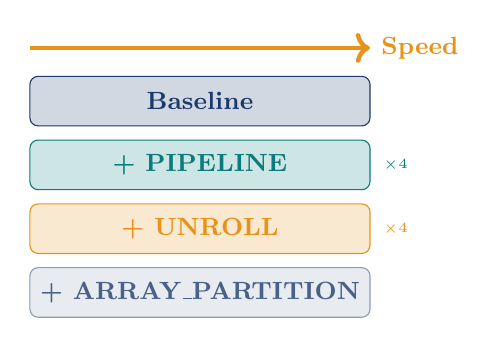
\begin{tikzpicture}[scale=0.9,font=\small]
    \draw[->,line width=1.6pt,color=Orange]
      (0,3.6) -- (4.8,3.6) node[right]{\color{Orange}\bfseries Speed};
    \filldraw[fill=Navy!20,draw=Navy,rounded corners=3pt]
      (0,2.5) rectangle (4.8,3.2) node[midway]{\color{Navy}\bfseries Baseline};
    \filldraw[fill=Teal!20,draw=Teal,rounded corners=3pt]
      (0,1.6) rectangle (4.8,2.3) node[midway]{\color{Teal}\bfseries + PIPELINE};
    \filldraw[fill=Orange!20,draw=Orange,rounded corners=3pt]
      (0,0.7) rectangle (4.8,1.4) node[midway]{\color{Orange}\bfseries + UNROLL};
    \filldraw[fill=Navy!10,draw=Navy!50,rounded corners=3pt]
      (0,-0.2) rectangle (4.8,0.5) node[midway]{\color{Navy!80}\bfseries + ARRAY\_PARTITION};
    \node[right,font=\tiny\color{Teal}]    at (4.85,1.95) {$\times4$};
    \node[right,font=\tiny\color{Orange}]  at (4.85,1.05) {$\times4$};
  \end{tikzpicture}
\end{columns}
\end{frame}

%% ── SLIDE 10 : PIPELINE concept ──────────────────────────────
\begin{frame}{\texttt{HLS PIPELINE} --- Concept}
\vspace{0.15cm}
\begin{columns}[T,totalwidth=\textwidth]
  \column{0.48\textwidth}

  \textbf{\color{Navy}Without PIPELINE} \hfill {\small II\,=\,4}
  \vspace{4pt}

  \hspace{3mm}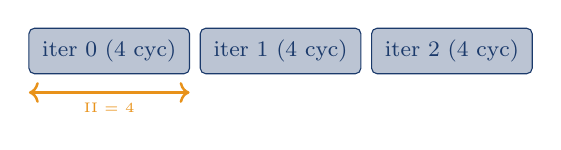
\begin{tikzpicture}[scale=0.68,font=\footnotesize]
    \foreach \i in {0,1,2}{
      \pgfmathsetmacro{\x}{\i*3.2}
      \filldraw[fill=Navy!30,draw=Navy,rounded corners=2pt]
        (\x,0) rectangle (\x+3.0,0.85);
      \node at (\x+1.5,0.425) {\color{Navy}iter \i\ (4 cyc)};
    }
    \draw[<->,color=Orange,line width=0.9pt] (0,-0.35)--(3.0,-0.35)
      node[midway,below,font=\tiny]{\color{Orange}II = 4};
  \end{tikzpicture}

  \vspace{10pt}
  \textbf{\color{Navy}With \texttt{PIPELINE}} \hfill {\small II\,=\,1 (no loop-carried dep.)}
  \vspace{4pt}

  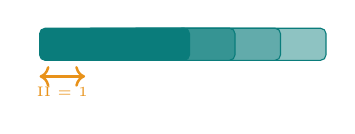
\begin{tikzpicture}[scale=0.68,font=\footnotesize]
    % 4 overlapping pipeline stages — each 2.8 wide, offset by 0.85
    \foreach \i in {3,2,1,0}{
      \pgfmathsetmacro{\x}{\i*0.85}
      \pgfmathsetmacro{\op}{100-\i*18}
      \filldraw[fill=Teal!\op!white,draw=Teal,rounded corners=2pt]
        (\x,0) rectangle (\x+2.8,0.6);
      \node[font=\tiny,text=Teal] at (\x+1.4,0.3) {it.\i};
    }
    \draw[<->,color=Orange,line width=0.9pt] (0,-0.3)--(0.85,-0.3)
      node[midway,below,font=\tiny]{\color{Orange}II = 1};
  \end{tikzpicture}

  {\fontsize{6.5}{8}\selectfont\color{MidGray}\itshape
   II\,=\,1 only when output does not feed back into the next iteration.\\
   Float accumulation (\texttt{acc\,+=\,...}) gives II\,=\,4 (FP adder latency).}

  \column{0.50\textwidth}
  \vspace{0.1cm}
  \colorbox{Navy!8}{\parbox{\dimexpr\linewidth-2\fboxsep\relax}{\vspace{4pt}
    \texttt{\#pragma HLS PIPELINE II=1}\\[2pt]
    {\small Place inside the loop body.}
  \vspace{4pt}}}

  \vspace{8pt}
  \begin{tabular}{lp{4.5cm}}
    \hline
    \rowcolor{Navy!10}\textbf{Param} & \textbf{Meaning}\\
    \hline
    \texttt{II=N}          & Target II (default 1)\\
    \rowcolor{Navy!5}\texttt{rewind}  & Overlap last/first iteration\\
    \texttt{enable\_flush} & Drain pipeline on stall\\
    \hline
  \end{tabular}

  \vspace{10pt}
  {\small\color{Orange}\bfseries Rule of thumb:} {\small start with the innermost loop.}
\end{columns}
\end{frame}

%% ── SLIDE 11 : PIPELINE applied ──────────────────────────────
\begin{frame}[fragile]{\texttt{PIPELINE} Applied to GEMM}
\vspace{0.1cm}
\begin{columns}[T,totalwidth=\textwidth]
  \column{0.46\textwidth}
\begin{lstlisting}
for(int i=0;i<N;i++)
 for(int j=0;j<N;j++){
  float acc=0;
  for(int k=0;k<N;k++){
   #pragma HLS PIPELINE
   acc+=A[i][k]*B[k][j];
  }
  C[i][j]=acc;
 }
\end{lstlisting}

  \column{0.52\textwidth}
  \vspace{0.1cm}
  {\small\color{Navy}\bfseries Synthesis report:}
  \vspace{4pt}

  \begin{tabular}{lll}
    \hline
    \rowcolor{Navy!10}\textbf{Loop} & \textbf{II} & \textbf{Latency}\\
    \hline
    inner \texttt{k}       & \textbf{\color{Orange}4} & 259 cyc\\
    \rowcolor{Navy!5}middle \texttt{j} & --- & $64^2\times259$\\
    outer \texttt{i}       & --- & $64^3\times259$\\
    \hline
  \end{tabular}

  \vspace{10pt}
  \colorbox{Teal!10}{\parbox{\dimexpr\linewidth-2\fboxsep\relax}{\vspace{4pt}
    {\color{Orange}\bfseries ${\approx}1.7\times$ speedup (FP dep.\ limits II)}\\
    {\small $1{,}835{,}008 \to 1{,}060{,}864$ cycles\\
    $18.4\,\text{ms} \to 10.6\,\text{ms}$ @ 100\,MHz}
  \vspace{4pt}}}
\end{columns}
\end{frame}

%% ── SLIDE 12 : UNROLL ────────────────────────────────────────
\begin{frame}[fragile]{\texttt{HLS UNROLL} --- Loop Unrolling}
\vspace{0.15cm}
\begin{columns}[T,totalwidth=\textwidth]
  \column{0.48\textwidth}

  \colorbox{Navy!8}{\parbox{\dimexpr\linewidth-2\fboxsep\relax}{\vspace{4pt}
    \texttt{\#pragma HLS UNROLL factor=F}\\[2pt]
    {\small $F$ iterations execute in parallel each cycle.}
  \vspace{4pt}}}

  \vspace{8pt}
  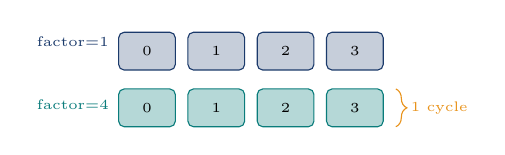
\begin{tikzpicture}[scale=0.80,font=\footnotesize]
    \node[left,font=\tiny\color{Navy}] at (0,1.25) {factor=1};
    \foreach \i in {0,1,2,3}{
      \pgfmathsetmacro{\x}{\i*1.1}
      \filldraw[fill=Navy!25,draw=Navy,rounded corners=2pt]
        (\x,0.8) rectangle (\x+0.9,1.4);
      \node[font=\tiny] at (\x+0.45,1.1) {\i};
    }
    \node[left,font=\tiny\color{Teal}] at (0,0.25) {factor=4};
    \foreach \i in {0,1,2,3}{
      \pgfmathsetmacro{\x}{\i*1.1}
      \filldraw[fill=Teal!30,draw=Teal,rounded corners=2pt]
        (\x,-0.1) rectangle (\x+0.9,0.5);
      \node[font=\tiny] at (\x+0.45,0.2) {\i};
    }
    \draw[decorate,decoration={brace,amplitude=4pt},color=Orange]
      (4.4,0.5) -- (4.4,-0.1)
      node[midway,right,font=\tiny,color=Orange]{\;1 cycle};
  \end{tikzpicture}

  \vspace{8pt}
  {\small\color{Orange}\bfseries Cost:} {\small LUT/DSP $\times F$.}

  \column{0.50\textwidth}
  \vspace{0.1cm}
\begin{lstlisting}
for(int k=0;k<N;k++){
  #pragma HLS PIPELINE II=1
  #pragma HLS UNROLL factor=4
  acc+=A[i][k]*B[k][j];
}
\end{lstlisting}

  \vspace{8pt}
  \begin{tabular}{lcc}
    \hline
    \rowcolor{Navy!10}\textbf{Config} & \textbf{II} & \textbf{k-lat.}\\
    \hline
    Baseline          & 7 & 448\\
    \rowcolor{Navy!5}+ PIPELINE        & 4 & 259\\
    + UNROLL$\times$4 & \textbf{\color{Teal}4} & \textbf{\color{Teal}70}\\
    \hline
  \end{tabular}
\end{columns}
\end{frame}

%% ── SLIDE 13 : ARRAY_PARTITION ───────────────────────────────
\begin{frame}[fragile]{\texttt{HLS ARRAY\_PARTITION} --- Memory Bottleneck}
\vspace{0.1cm}
\begin{columns}[T,totalwidth=\textwidth]
  \column{0.50\textwidth}

  {\small\color{Navy}\bfseries Problem:} BRAMs have \textbf{2 ports max}.
  Unrolled loop needs $F$ reads/cycle --- HLS raises II.

  \vspace{5pt}
  \colorbox{Navy!8}{\parbox{\dimexpr\linewidth-2\fboxsep\relax}{\vspace{3pt}
    {\fontsize{8}{10}\selectfont\ttfamily\#pragma HLS ARRAY\_PARTITION}\\
    {\fontsize{8}{10}\selectfont\ttfamily\ \ variable=A dim=2 factor=4 cyclic}\\[1pt]
    {\footnotesize \textbf{cyclic}: interleaved \quad
            \textbf{block}: contiguous \quad
            \textbf{complete}: full registers}
  \vspace{3pt}}}

  \vspace{3pt}
  \colorbox{BoxGray!12}{\parbox{\dimexpr\linewidth-2\fboxsep\relax}{\vspace{2pt}
    {\fontsize{8}{10}\selectfont\ttfamily\#pragma HLS ARRAY\_RESHAPE}\\
    {\footnotesize \textbf{Wider word}, fewer BRAMs — same bandwidth as partition.}
  \vspace{2pt}}}

  \vspace{5pt}
  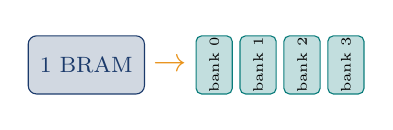
\begin{tikzpicture}[scale=0.82,font=\footnotesize]
    \filldraw[fill=Navy!20,draw=Navy,rounded corners=3pt]
      (0,0) rectangle (1.8,0.9) node[midway]{\color{Navy}1 BRAM};
    \node at (2.2,0.45) {\large\color{Orange}$\to$};
    \foreach \i in {0,1,2,3}{
      \pgfmathsetmacro{\x}{2.6+\i*0.68}
      \filldraw[fill=Teal!25,draw=Teal,rounded corners=2pt]
        (\x,0) rectangle (\x+0.56,0.9);
      \node[font=\tiny,rotate=90] at (\x+0.28,0.45) {bank \i};
    }
  \end{tikzpicture}

  \column{0.48\textwidth}
  \vspace{0.1cm}
\begin{lstlisting}[basicstyle=\ttfamily\scriptsize]
#pragma HLS ARRAY_PARTITION
  variable=A factor=4 cyclic dim=2
#pragma HLS ARRAY_PARTITION
  variable=B factor=4 cyclic dim=1
\end{lstlisting}

  \vspace{8pt}
  \begin{tabular}{lcc}
    \hline
    \rowcolor{Navy!10}\textbf{Config} & \textbf{II} & \textbf{Speed}\\
    \hline
    Baseline              & 7 & $1\times$\\
    \rowcolor{Navy!5}+ PIPELINE            & 4 & ${\approx}1.7\times$\\
    + UNROLL, no PART.    & \textbf{4!} & stalled\\
    \rowcolor{Navy!5}+ PART.\ + ap\_fixed  & \textbf{\color{Teal}1} & $\mathbf{7\times}$\\
    \hline
  \end{tabular}
\end{columns}
\end{frame}

%% ── SLIDE 14 : DATAFLOW ───────────────────────────────────────
\begin{frame}[fragile]{\texttt{HLS DATAFLOW} --- Task-Level Pipelining}
\vspace{0.1cm}
\begin{columns}[T,totalwidth=\textwidth]
  \column{0.50\textwidth}

  {\small Overlaps \emph{sequential functions} --- producer/consumer at the task level.}

  \vspace{8pt}
  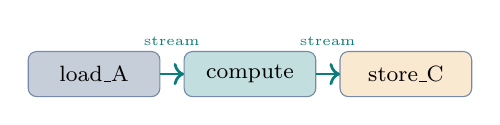
\begin{tikzpicture}[scale=0.88,font=\footnotesize]
    \def\bw{1.9}\def\bh{0.65}\def\gap{0.35}
    \foreach \i/\fname/\col in {
        0/{load\_A}/Navy!25,
        1/compute/Teal!25,
        2/{store\_C}/Orange!20}{
      \pgfmathsetmacro{\x}{\i*(\bw+\gap)}
      \filldraw[fill=\col,draw=Navy!60,rounded corners=3pt]
        (\x,0) rectangle (\x+\bw,\bh);
      \node at (\x+\bw/2,\bh/2) {\fname};
    }
    \draw[->,line width=1pt,color=Teal]
      (1.9,\bh/2) -- (2.25,\bh/2);
    \draw[->,line width=1pt,color=Teal]
      (4.15,\bh/2) -- (4.5,\bh/2);
    \node[font=\tiny,color=Teal] at (2.07,\bh+0.15) {stream};
    \node[font=\tiny,color=Teal] at (4.32,\bh+0.15) {stream};
  \end{tikzpicture}

  \vspace{8pt}
  \colorbox{Navy!8}{\parbox{\dimexpr\linewidth-2\fboxsep\relax}{\vspace{4pt}
    \texttt{\#pragma HLS DATAFLOW}\\[2pt]
    {\small Place at the top-level function.\\
    Use \texttt{hls::stream<>} between stages.}
  \vspace{4pt}}}

  \column{0.48\textwidth}
  \vspace{0.1cm}
\begin{lstlisting}
void top(data_t in[],
         data_t out[]){
  #pragma HLS DATAFLOW
  hls::stream<data_t> s1,s2;
  load(in,  s1);
  compute(s1, s2);
  store(s2, out);
}
\end{lstlisting}

  \vspace{8pt}
  \colorbox{Teal!10}{\parbox{\dimexpr\linewidth-2\fboxsep\relax}{\vspace{4pt}
    {\color{Teal}\bfseries Interval} = max(stage II), not sum.
  \vspace{4pt}}}

  \vspace{6pt}
  {\small Use when:\ streaming I/O, multi-stage pipelines, DMA + compute overlap.}
\end{columns}
\end{frame}

%% ── SLIDE 15 : Pragma interaction guidelines ─────────────────
\begin{frame}{Pragma Interaction \& Guidelines}
\vspace{0.15cm}
\begin{columns}[T,totalwidth=\textwidth]
  \column{0.50\textwidth}

  \begin{tabular}{p{3.0cm}p{3.4cm}}
    \hline
    \rowcolor{Navy!10}\textbf{Situation} & \textbf{Pragma}\\
    \hline
    Loop-carried dep.\ limits II & \texttt{PIPELINE}\\
    \hline
    \rowcolor{Navy!5}Need $F\!\times$ throughput & \texttt{UNROLL factor=F}\\
    \rowcolor{Navy!5}\quad Too much area          & \quad reduce \texttt{factor}\\
    \hline
    Memory port conflict         & \texttt{ARRAY\_PARTITION}\\
    \hline
    Sequential stages            & \texttt{DATAFLOW}\\
    \hline
  \end{tabular}

  \vspace{10pt}
  \colorbox{Orange!10}{\parbox{\dimexpr\linewidth-2\fboxsep\relax}{\raggedright\vspace{4pt}
    {\color{Orange}\bfseries Always pair \mbox{UNROLL\,+\,PARTITION}.}\\[2pt]
    {\small Unrolling alone serialises memory accesses.}
  \vspace{4pt}}}

  \column{0.48\textwidth}
  \vspace{0.2cm}
  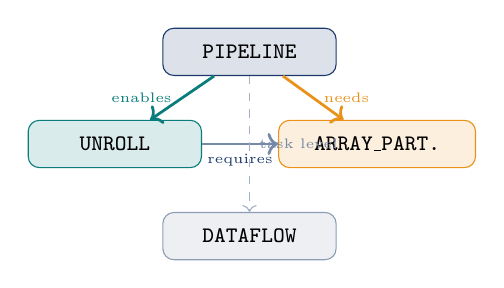
\begin{tikzpicture}[scale=0.90,font=\footnotesize]
    \node[draw=Navy,fill=Navy!15,rounded corners=4pt,
          minimum width=2.2cm,minimum height=0.6cm]
      (pip) at (2.1,3.0) {\texttt{PIPELINE}};
    \node[draw=Teal,fill=Teal!15,rounded corners=4pt,
          minimum width=2.2cm,minimum height=0.6cm]
      (unr) at (0.2,1.7) {\texttt{UNROLL}};
    \node[draw=Orange,fill=Orange!15,rounded corners=4pt,
          minimum width=2.5cm,minimum height=0.6cm]
      (par) at (3.9,1.7) {\texttt{ARRAY\_PART.}};
    \node[draw=Navy!50,fill=Navy!8,rounded corners=4pt,
          minimum width=2.2cm,minimum height=0.6cm]
      (dat) at (2.1,0.4) {\texttt{DATAFLOW}};
    \draw[->,color=Teal,line width=1pt] (pip)--(unr)
      node[midway,left,font=\tiny,color=Teal]{enables};
    \draw[->,color=Orange,line width=1pt] (pip)--(par)
      node[midway,right,font=\tiny,color=Orange]{needs};
    \draw[->,color=Navy!60,line width=1pt] (unr)--(par)
      node[midway,below,font=\tiny,color=Navy]{requires};
    \draw[->,color=Navy!40,dashed] (pip)--(dat)
      node[midway,right,font=\tiny,color=Navy!60]{task level};
  \end{tikzpicture}
\end{columns}
\end{frame}

%% ── SLIDE 16 : Reading the synthesis report ──────────────────
\begin{frame}{Reading the Vitis HLS Synthesis Report}
\vspace{0.15cm}
\begin{columns}[T,totalwidth=\textwidth]
  \column{0.50\textwidth}

  \begin{tabular}{p{2.5cm}p{4.2cm}}
    \hline
    \rowcolor{Navy!10}\textbf{Field} & \textbf{What to check}\\
    \hline
    \texttt{Target II}     & What you requested\\
    \hline
    \rowcolor{Navy!5}\texttt{Achieved II}  & What HLS managed\\
    \hline
    \texttt{Violation}     & Dep.\ or resource conflict\\
    \hline
    \rowcolor{Navy!5}\texttt{BRAM/DSP/LUT} & Resource budget\\
    \hline
    \texttt{Slack}         & Timing ($\geq 0$)\\
    \hline
  \end{tabular}

  \vspace{10pt}
  \colorbox{Teal!10}{\parbox{\dimexpr\linewidth-2\fboxsep\relax}{\vspace{4pt}
    {\color{Teal}\bfseries In Vitis HLS GUI:}\\
    {\small Solution $\to$ Open Report $\to$ Synthesis\\
    \textbf{Loop} tab: per-loop II and latency}
  \vspace{4pt}}}

  \column{0.48\textwidth}
  \vspace{0.1cm}
  \colorbox{Orange!10}{\parbox{\dimexpr\linewidth-2\fboxsep\relax}{\vspace{4pt}
    {\color{Orange}\bfseries Workflow:}\\[4pt]
    {\small
    1.\ Synthesise without pragmas\\[2pt]
    2.\ Add \texttt{PIPELINE II=1}, check achieved II\\[2pt]
    3.\ II $>$ 1? Check Violation:\\
    \hspace{8pt}$\bullet$\ FP dep.\ $\to$ DSP chaining\\
    \hspace{8pt}$\bullet$\ Memory $\to$ \texttt{ARRAY\_PARTITION}\\[2pt]
    4.\ Add \texttt{UNROLL}, re-check area}
  \vspace{4pt}}}
\end{columns}
\end{frame}

%% ── SLIDE 17 : Fully optimised GEMM ─────────────────────────
\begin{frame}[fragile]{Best Float Performance}
\vspace{0.1cm}
\begin{columns}[T,totalwidth=\textwidth]
  \column{0.52\textwidth}
\begin{lstlisting}[basicstyle=\ttfamily\scriptsize]
void gemm(float A[N][N],
          float B[N][N],
          float C[N][N]){
#pragma HLS ARRAY_PARTITION
  variable=A factor=4 cyclic dim=2
#pragma HLS ARRAY_PARTITION
  variable=B factor=4 cyclic dim=1
  for(int i=0;i<N;i++)
   for(int j=0;j<N;j++){
    float acc=0;
    for(int k=0;k<N;k++){
     #pragma HLS PIPELINE II=1
     #pragma HLS UNROLL factor=4
     acc+=A[i][k]*B[k][j];
    }
    C[i][j]=acc;
   }
}
\end{lstlisting}

  \column{0.46\textwidth}
  \vspace{0.2cm}
  \begin{tabular}{p{2.6cm}cc}
    \hline
    \rowcolor{Navy!10}\textbf{Version} & \textbf{Cycles} & \textbf{Time}\\
    \hline
    Baseline                  & $1{,}835{,}008$ & $18.4$\,ms\\
    \rowcolor{Navy!5}+ PIPELINE (II=4) & $1{,}060{,}864$ & $10.6$\,ms\\
    + UNROLL$\times$4         & $\approx 307{,}200$ & $\approx 3.1$\,ms\\
    \rowcolor{Navy!5}+ PARTITION       & \textbf{\color{Teal}$\approx 307{,}200$} & \textbf{\color{Teal}$\approx 3.1$\,ms}\\
    \hline
  \end{tabular}

  \vspace{10pt}
  \colorbox{Navy!8}{\parbox{\dimexpr\linewidth-2\fboxsep\relax}{\vspace{4pt}
    {\small DSP48: $\approx$36 \quad BRAM: $\approx$6 \quad LUT: $\approx4\times$}
  \vspace{4pt}}}

  \vspace{6pt}
  {\small\color{Navy!70}\itshape $\mathbf{{\approx}7\times}$ speedup (float, II=4), $4\times$ resources. ap\_fixed gives another $4\times$.}
\end{columns}
\end{frame}

%% ── SLIDE 18 : Section 3 key takeaways ───────────────────────
\begin{frame}{Loop Optimisation Pragmas --- Key Takeaways}
\vspace{0.15cm}
\begin{columns}[T,totalwidth=\textwidth]
  \column{0.50\textwidth}

  \colorbox{Navy!8}{\parbox{\dimexpr\linewidth-2\fboxsep\relax}{\vspace{4pt}
    \textbf{\color{Navy}1.\ PIPELINE} --- overlap iterations, target II=1
  \vspace{4pt}}}
  \vspace{5pt}

  \colorbox{Teal!10}{\parbox{\dimexpr\linewidth-2\fboxsep\relax}{\vspace{4pt}
    \textbf{\color{Teal}2.\ UNROLL} --- $F$ iterations in parallel, $F\times$ area
  \vspace{4pt}}}
  \vspace{5pt}

  \colorbox{Orange!10}{\parbox{\dimexpr\linewidth-2\fboxsep\relax}{\vspace{4pt}
    \textbf{\color{Orange}3.\ ARRAY\_PARTITION} --- split BRAM into $F$ banks
  \vspace{4pt}}}
  \vspace{5pt}

  \colorbox{Navy!8}{\parbox{\dimexpr\linewidth-2\fboxsep\relax}{\vspace{4pt}
    \textbf{\color{Navy}4.\ DATAFLOW} --- overlap sequential functions
  \vspace{4pt}}}

  \column{0.48\textwidth}
  \vspace{0.2cm}
  \begin{tabular}{lcc}
    \hline
    \rowcolor{Navy!10}\textbf{Pragma} & \textbf{II effect} & \textbf{Area}\\
    \hline
    PIPELINE          & II$\to$min dep. (4 for FP) & $+$FF\\
    \rowcolor{Navy!5}UNROLL$\times F$ & $\downarrow F\times$ & $\uparrow F\times$\\
    ARRAY\_PART.      & enables above & +BRAM\\
    \rowcolor{Navy!5}DATAFLOW         & task overlap & minor\\
    \hline
  \end{tabular}

  \vspace{12pt}
  {\color{Orange}\bfseries Golden rule:} {\small measure first, then add pragmas.}
\end{columns}
\end{frame}

%% ════════════════════════════════════════════════════════════
%%  SECTION 4 --- Resources & Timing
%% ════════════════════════════════════════════════════════════

%% ── SLIDE 19 : Section header ────────────────────────────────
\begin{frame}{Section 4 --- Resources \& Timing}
\vspace{0.2cm}
\begin{columns}[T,totalwidth=\textwidth]
  \column{0.52\textwidth}

  \colorbox{Navy!8}{\parbox{\dimexpr\linewidth-2\fboxsep\relax}{\vspace{5pt}
    \textbf{What we cover:}\\[4pt]
    \hspace{6pt}$\bullet$\ FPGA resource types (LUT, DSP, BRAM, FF)\\[2pt]
    \hspace{6pt}$\bullet$\ How HLS maps C operators to resources\\[2pt]
    \hspace{6pt}$\bullet$\ Reading the utilisation report\\[2pt]
    \hspace{6pt}$\bullet$\ Clock constraint \& timing closure
  \vspace{5pt}}}

  \vspace{10pt}
  {\small\color{MidGray}\itshape Pragmas change speed --- but they also change
  area. Understanding both is essential.}

  \column{0.46\textwidth}
  \vspace{0.3cm}
  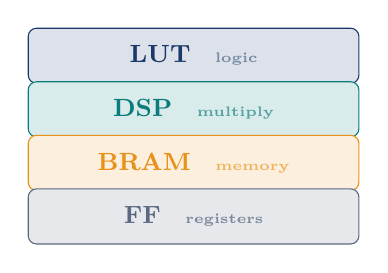
\begin{tikzpicture}[scale=0.85,font=\small]
    \node[draw=Navy,fill=Navy!15,rounded corners=3pt,
          minimum width=4.2cm,minimum height=0.7cm,align=center]
      at (0,2.4) {\color{Navy}\bfseries LUT \enspace{\tiny\color{Navy!60}logic}};
    \node[draw=Teal,fill=Teal!15,rounded corners=3pt,
          minimum width=4.2cm,minimum height=0.7cm,align=center]
      at (0,1.6) {\color{Teal}\bfseries DSP \enspace{\tiny\color{Teal!70}multiply}};
    \node[draw=Orange,fill=Orange!15,rounded corners=3pt,
          minimum width=4.2cm,minimum height=0.7cm,align=center]
      at (0,0.8) {\color{Orange}\bfseries BRAM \enspace{\tiny\color{Orange!70}memory}};
    \node[draw=BoxGray,fill=BoxGray!15,rounded corners=3pt,
          minimum width=4.2cm,minimum height=0.7cm,align=center]
      at (0,0.0) {\color{BoxGray}\bfseries FF \enspace{\tiny\color{BoxGray!80}registers}};
  \end{tikzpicture}
\end{columns}
\end{frame}

%% ── SLIDE 20 : FPGA Resources ────────────────────────────────
\begin{frame}{FPGA Resource Types}
\vspace{0.1cm}
\begin{columns}[T,totalwidth=\textwidth]

  \column{0.49\textwidth}

  \colorbox{Navy!8}{\parbox{\dimexpr\linewidth-2\fboxsep\relax}{\vspace{4pt}
    {\color{Navy}\bfseries LUT} — Look-Up Table\\[2pt]
    {\small Implements any Boolean function of $\leq$6 inputs.
    Used for logic, muxes, adders, comparators.}
  \vspace{4pt}}}
  \vspace{5pt}

  \colorbox{Teal!10}{\parbox{\dimexpr\linewidth-2\fboxsep\relax}{\vspace{4pt}
    {\color{Teal}\bfseries DSP48E} — Multiply-Accumulate block\\[2pt]
    {\small Hard 18$\times$27-bit multiplier + adder.
    HLS infers these automatically for \texttt{*} and \texttt{MAC}.}
  \vspace{4pt}}}
  \vspace{5pt}

  \colorbox{Orange!10}{\parbox{\dimexpr\linewidth-2\fboxsep\relax}{\vspace{4pt}
    {\color{Orange}\bfseries BRAM\_18K} — Block RAM\\[2pt]
    {\small 18\,Kb dual-port RAM. Arrays $>$ a few elements
    are mapped here by HLS.}
  \vspace{4pt}}}

  \column{0.02\textwidth}

  \column{0.49\textwidth}
  \vspace{0.1cm}

  \colorbox{BoxGray!10}{\parbox{\dimexpr\linewidth-2\fboxsep\relax}{\vspace{4pt}
    {\color{BoxGray}\bfseries FF} — Flip-Flop\\[2pt]
    {\small 1-bit register. Used for pipeline registers,
    interface signals, state machines.}
  \vspace{4pt}}}

  \vspace{10pt}
  {\small\color{Navy}\bfseries Rough cost per operator:}
  \vspace{4pt}

  \begin{tabular}{lp{3.8cm}}
    \hline
    \rowcolor{Navy!10}\textbf{Operator} & \textbf{Typical cost}\\
    \hline
    \texttt{int} add/cmp  & $\sim$1 LUT/bit\\
    \rowcolor{Navy!5}\texttt{int} mul    & 1--3 DSP48E\\
    FP add (32-bit)       & $\sim$400 LUT, 2 DSP\\
    \rowcolor{Navy!5}FP mul (32-bit)    & $\sim$3 DSP48E\\
    \hline
  \end{tabular}

\end{columns}
\end{frame}

%% ── SLIDE 21 : Reading the Utilisation Report ─────────────────
\begin{frame}{Reading the Utilisation Report}
\vspace{0.05cm}
\begin{columns}[T,totalwidth=\textwidth]

  \column{0.54\textwidth}
  {\small\color{Navy}\bfseries Vitis HLS — Utilization Estimates:}
  \vspace{3pt}

  \colorbox{NavyDk!6}{\parbox{\dimexpr\linewidth-2\fboxsep\relax}{
  \ttfamily\fontsize{7.5}{10}\selectfont\color{NavyDk}
  + Utilization Estimates\\
  \hspace{1em}+ Summary\\
  \hspace{2em}Name      : gemm\\
  \hspace{2em}BRAM\_18K : \textbf{\color{Orange}6}\\
  \hspace{2em}DSP48E    : \textbf{\color{Teal}9}\\
  \hspace{2em}FF        : 1204\\
  \hspace{2em}LUT       : \textbf{\color{Navy}3841}\\[4pt]
  \hspace{1em}+ Details\\
  \hspace{2em}* A[64][64] -> BRAM x2\\
  \hspace{2em}* B[64][64] -> BRAM x2\\
  \hspace{2em}* C[64][64] -> BRAM x2\\
  \hspace{2em}* fmul\_32ns -> DSP48E x3\\
  \hspace{2em}* fadd\_32ns -> DSP48E x6
  }}

  \column{0.44\textwidth}
  \vspace{0.2cm}

  \colorbox{Orange!10}{\parbox{\dimexpr\linewidth-2\fboxsep\relax}{\vspace{3pt}
    {\color{Orange}\bfseries 6 BRAM} — one per matrix\\
    {\small Each 64$\times$64 float = 16\,KB $>$ 1 BRAM\_18K, so HLS uses 2 per array.}
  \vspace{3pt}}}

  \vspace{8pt}
  \colorbox{Teal!10}{\parbox{\dimexpr\linewidth-2\fboxsep\relax}{\vspace{3pt}
    {\color{Teal}\bfseries 9 DSP} — FP operators\\
    {\small FP mul = 3 DSP, FP add = 6 DSP. Float is expensive.}
  \vspace{3pt}}}

  \vspace{8pt}
  {\small\color{Navy}Check against your device budget.\\
  Zynq-7020: 220 DSP, 140 BRAM — plenty here.}

\end{columns}
\end{frame}

%% ── SLIDE 22 : Clock Constraint & Timing Closure ─────────────
\begin{frame}{Clock Constraint \& Timing Closure}
\vspace{0.1cm}
\begin{columns}[T,totalwidth=\textwidth]

  \column{0.49\textwidth}

  \colorbox{Navy!8}{\parbox{\dimexpr\linewidth-2\fboxsep\relax}{\vspace{4pt}
    {\color{Navy}\bfseries Set the clock in the HLS solution:}\\[3pt]
    {\small Target period = 10\,ns $\Rightarrow$ 100\,MHz.\\
    HLS adds pipeline registers to meet timing.}
  \vspace{4pt}}}

  \vspace{8pt}
  {\small\color{Navy}What HLS reports:}
  \vspace{3pt}

  \colorbox{NavyDk!6}{\parbox{\dimexpr\linewidth-2\fboxsep\relax}{
  \ttfamily\fontsize{7.5}{10}\selectfont\color{NavyDk}
  + Timing (ns)\\
  \hspace{1em}* Summary\\
  \hspace{2em}Clock target   : 10.00\\
  \hspace{2em}Estimated      : \textbf{\color{Teal}8.24}\\
  \hspace{2em}Uncertainty    : 1.25
  }}

  \vspace{8pt}
  {\small\color{GreenHi}Estimated $<$ target: timing met.}

  \column{0.02\textwidth}

  \column{0.49\textwidth}
  \vspace{0.1cm}

  \colorbox{Orange!10}{\parbox{\dimexpr\linewidth-2\fboxsep\relax}{\vspace{4pt}
    {\color{Orange}\bfseries If estimated $>$ target:}\\[2pt]
    {\small HLS still generates RTL but flags a warning.
    Vivado implementation may then fail timing — reduce
    the clock or simplify the datapath.}
  \vspace{4pt}}}

  \vspace{8pt}
  {\small\color{Navy}Typical causes of timing failure:}
  \begin{itemize}\setlength{\itemsep}{1pt}
    {\small
    \item FP operators on critical path
    \item Wide multipliers not absorbed by DSP
    \item Long combinational mux trees}
  \end{itemize}

\end{columns}
\end{frame}

%% ── SLIDE 23 : Resources vs Speed Trade-off ──────────────────
\begin{frame}{Resources vs.\ Speed: the Trade-off}
\vspace{0.1cm}
\begin{columns}[T,totalwidth=\textwidth]

  \column{0.49\textwidth}

  \begin{tabular}{p{2.6cm}p{1.2cm}p{1.6cm}}
    \hline
    \rowcolor{Navy!10}\textbf{Action} & \textbf{Speed} & \textbf{Area}\\
    \hline
    \texttt{PIPELINE}      & $\uparrow\uparrow$ & $+$FF regs\\
    \rowcolor{Navy!5}\texttt{UNROLL}$\times F$ & $\uparrow F\times$ & $\uparrow F\times$\\
    \texttt{ARRAY\_PART.}  & enables UNR & +BRAM\\
    \rowcolor{Navy!5}\texttt{float}$\to$\texttt{int} & $\uparrow\uparrow$ & $\downarrow\downarrow$\\
    Reduce clock           & $\downarrow$ & $\searrow$\\
    \hline
  \end{tabular}

  \vspace{10pt}
  {\color{Orange}\bfseries\small Rule:} {\small PIPELINE first — FF overhead is small.
  UNROLL only if you have DSP/BRAM headroom.}

  \column{0.02\textwidth}

  \column{0.49\textwidth}
  \vspace{0.1cm}

  \colorbox{Teal!10}{\parbox{\dimexpr\linewidth-2\fboxsep\relax}{\vspace{4pt}
    {\color{Teal}\bfseries Typical workflow:}\\[3pt]
    {\small
    1.\ Compile baseline, note II \& area.\\[2pt]
    2.\ Add \texttt{PIPELINE} to inner loop.\\[2pt]
    3.\ Check report — II met?\\[2pt]
    4.\ Memory bottleneck? Add \texttt{ARRAY\_PART.}\\[2pt]
    5.\ If still slow: \texttt{UNROLL}, watch area.\\[2pt]
    6.\ Verify timing in Vivado.}
  \vspace{4pt}}}

\end{columns}
\end{frame}

%% ════════════════════════════════════════════════════════════
%%  SECTION 5 --- Connecting to the Lab
%% ════════════════════════════════════════════════════════════

%% ── SLIDE 24 : Section header ────────────────────────────────
\begin{frame}{Section 5 --- Connecting to the Lab}
\vspace{0.15cm}
\begin{columns}[T,totalwidth=\textwidth]
  \column{0.54\textwidth}

  \colorbox{Navy!8}{\parbox{\dimexpr\linewidth-2\fboxsep\relax}{\vspace{5pt}
    \textbf{Lab goal:} apply today's pragmas to a\\
    real GEMM HLS IP and measure the effect.\\[6pt]
    \hspace{6pt}$\bullet$\ Baseline inner loop --- II\,=\,7\\[2pt]
    \hspace{6pt}$\bullet$\ Add \texttt{PIPELINE} --- II\,=\,4 (FP dep.)\\[2pt]
    \hspace{6pt}$\bullet$\ Add \texttt{UNROLL} + \texttt{ARRAY\_PARTITION}\\[2pt]
    \hspace{6pt}$\bullet$\ Read the synthesis report each time
  \vspace{5pt}}}

  \vspace{8pt}
  {\small\color{MidGray}\itshape You already have the AXI-Stream interface
  from L5. Today you optimise what's inside the IP.}

  \column{0.44\textwidth}
  \vspace{0.2cm}
  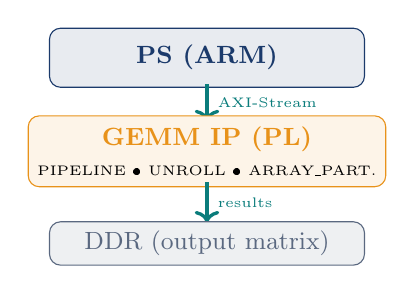
\begin{tikzpicture}[scale=0.88,font=\small]
    \node[draw=Navy,fill=Navy!10,rounded corners=4pt,
          minimum width=4.0cm,minimum height=0.75cm,align=center]
      at (0,3.2) {\color{Navy}\bfseries PS (ARM)};
    \draw[->,line width=1.2pt,color=Teal] (0,2.82) -- (0,2.28)
      node[midway,right,font=\tiny\color{Teal}]{AXI-Stream};
    \node[draw=Orange,fill=Orange!10,rounded corners=4pt,
          minimum width=4.0cm,minimum height=0.9cm,align=center]
      at (0,1.85) {\color{Orange}\bfseries GEMM IP (PL)\\
        {\tiny PIPELINE \textbullet\ UNROLL \textbullet\ ARRAY\_PART.}};
    \draw[->,line width=1.2pt,color=Teal] (0,1.4) -- (0,0.82)
      node[midway,right,font=\tiny\color{Teal}]{results};
    \node[draw=BoxGray,fill=BoxGray!10,rounded corners=4pt,
          minimum width=4.0cm,minimum height=0.55cm,align=center]
      at (0,0.52) {\color{BoxGray}\small DDR (output matrix)};
  \end{tikzpicture}
\end{columns}
\end{frame}

%% ── SLIDE 25 : Lab Steps ─────────────────────────────────────
\begin{frame}[fragile]{Lab Steps}
\vspace{0.05cm}
\begin{columns}[T,totalwidth=\textwidth]

  \column{0.48\textwidth}
  {\small\color{Navy}\bfseries Step 1 — Baseline (no pragmas):}
  \vspace{2pt}
\begin{lstlisting}
for(int k=0; k<N; k++)
  acc += A[i][k]*B[k][j];
\end{lstlisting}
  {\small Note II, latency, DSP, LUT in report.}

  \vspace{8pt}
  {\small\color{Navy}\bfseries Step 2 — Add PIPELINE:}
  \vspace{2pt}
\begin{lstlisting}
for(int k=0; k<N; k++){
  #pragma HLS PIPELINE II=1
  acc += A[i][k]*B[k][j];
}
\end{lstlisting}
  {\small Does II reach 1? Check the report.}

  \column{0.50\textwidth}
  \vspace{0.0cm}
  {\small\color{Navy}\bfseries Step 3 — Add UNROLL + ARRAY\_PARTITION:}
  \vspace{2pt}
\begin{lstlisting}
#pragma HLS ARRAY_PARTITION \
  variable=A cyclic factor=4
#pragma HLS ARRAY_PARTITION \
  variable=B cyclic factor=4
for(int k=0; k<N; k++){
  #pragma HLS PIPELINE II=1
  #pragma HLS UNROLL factor=4
  acc += A[i][k]*B[k][j];
}
\end{lstlisting}

  \vspace{4pt}
  \colorbox{Orange!10}{\parbox{\dimexpr\linewidth-2\fboxsep\relax}{\vspace{2pt}
    {\small\color{Orange}\bfseries Record II, latency \& DSP count
    after each step.}
  \vspace{2pt}}}

\end{columns}
\end{frame}

%% ── SLIDE 26 : Expected Results ──────────────────────────────
\begin{frame}{Expected Results}
\vspace{0.1cm}
\begin{columns}[T,totalwidth=\textwidth]

  \column{0.52\textwidth}

  \begin{tabular}{lp{0.5cm}p{0.7cm}p{1.0cm}}
    \hline
    \rowcolor{Navy!10}\textbf{Version} & \textbf{II} & \textbf{DSP} & \textbf{Speedup}\\
    \hline
    Baseline             & 7 & 9  & $1\times$\\
    \rowcolor{Navy!5}+\ PIPELINE (float) & 4 & 9  & ${\approx}1.7\times$\\
    +\ ap\_fixed + UNROLL$\times$4   & 1 & 36 & ${\approx}28\times$\\
    \hline
  \end{tabular}

  \vspace{10pt}
  {\small\color{Navy}If II\,$>$\,1 after PIPELINE, look for:}
  \begin{itemize}\setlength{\itemsep}{1pt}
    {\small
    \item Loop-carried FP dependency (expected)
    \item Memory port conflict (add ARRAY\_PART.)
    \item Report says ``II\,=\,4, target\,=\,1''}
  \end{itemize}

  \column{0.46\textwidth}
  \vspace{0.1cm}

  \colorbox{Teal!10}{\parbox{\dimexpr\linewidth-2\fboxsep\relax}{\vspace{4pt}
    {\color{Teal}\bfseries What to hand in:}\\[3pt]
    {\small
    $\bullet$\ Synthesis report screenshot per step\\[2pt]
    $\bullet$\ Table: II, latency, DSP per version\\[2pt]
    $\bullet$\ Brief explanation of why II changes}
  \vspace{4pt}}}

  \vspace{8pt}
  \colorbox{Orange!10}{\parbox{\dimexpr\linewidth-2\fboxsep\relax}{\vspace{4pt}
    {\color{Orange}\bfseries Common mistake:}\\[2pt]
    {\small UNROLL without ARRAY\_PARTITION ---
    memory ports stall the pipeline. Always pair them.}
  \vspace{4pt}}}

\end{columns}
\end{frame}

%% ════════════════════════════════════════════════════════════
%%  SECTION 6 --- Float vs Fixed
%% ════════════════════════════════════════════════════════════

%% ── SLIDE 27 : Section header ────────────────────────────────
\begin{frame}{Section 6 --- Float vs.\ Fixed}
\vspace{0.15cm}
\begin{columns}[T,totalwidth=\textwidth]
  \column{0.54\textwidth}

  \colorbox{Navy!8}{\parbox{\dimexpr\linewidth-2\fboxsep\relax}{\vspace{5pt}
    \textbf{What we cover:}\\[4pt]
    \hspace{6pt}$\bullet$\ What IEEE\,754 float actually is in HW\\[2pt]
    \hspace{6pt}$\bullet$\ Why float accumulation gives II\,=\,4\\[2pt]
    \hspace{6pt}$\bullet$\ \texttt{ap\_fixed<W,I>} --- format \& syntax\\[2pt]
    \hspace{6pt}$\bullet$\ Why fixed-point gives II\,=\,1\\[2pt]
    \hspace{6pt}$\bullet$\ Area, accuracy, and how to choose W, I
  \vspace{5pt}}}

  \vspace{8pt}
  {\small\color{MidGray}\itshape Float is convenient. Fixed is fast and small.
  Knowing the cost lets you choose.}

  \column{0.44\textwidth}
  \vspace{0.3cm}
  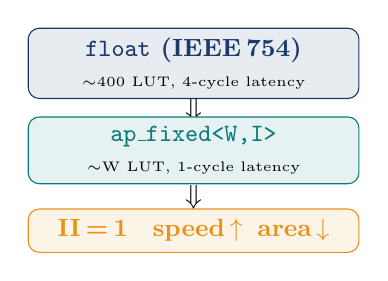
\begin{tikzpicture}[scale=0.85,font=\small]
    \node[draw=Navy,fill=Navy!10,rounded corners=4pt,
          minimum width=4.2cm,minimum height=0.75cm,align=center]
      at (0,2.4) {\color{Navy}\bfseries \texttt{float} (IEEE\,754)\\
        {\tiny $\sim$400 LUT, 4-cycle latency}};
    \node[font=\normalsize] at (0,1.7) {$\Downarrow$};
    \node[draw=Teal,fill=Teal!10,rounded corners=4pt,
          minimum width=4.2cm,minimum height=0.75cm,align=center]
      at (0,1.1) {\color{Teal}\bfseries \texttt{ap\_fixed<W,I>}\\
        {\tiny $\sim$W LUT, 1-cycle latency}};
    \node[font=\normalsize] at (0,0.4) {$\Downarrow$};
    \node[draw=Orange,fill=Orange!10,rounded corners=4pt,
          minimum width=4.2cm,minimum height=0.55cm,align=center]
      at (0,-0.1) {\color{Orange}\bfseries II\,=\,1 \enspace speed\,$\uparrow$\enspace area\,$\downarrow$};
  \end{tikzpicture}
\end{columns}
\end{frame}

%% ── SLIDE 28 : What IEEE 754 float is ───────────────────────
\begin{frame}{What IEEE\,754 Float Actually Is}
\vspace{0.1cm}
\begin{columns}[T,totalwidth=\textwidth]

  \column{0.52\textwidth}
  \vspace{0.1cm}

  {\small A 32-bit \texttt{float} is split into three fields:}
  \vspace{6pt}

  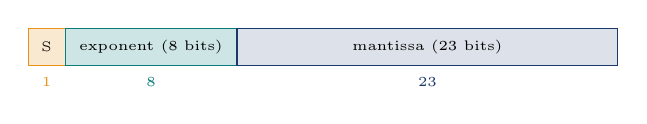
\begin{tikzpicture}[scale=0.78,font=\footnotesize]
    % bit fields
    \filldraw[fill=Orange!20,draw=Orange] (0,0) rectangle (0.6,0.6);
    \node at (0.3,0.3) {\tiny S};
    \filldraw[fill=Teal!20,draw=Teal]   (0.6,0) rectangle (3.4,0.6);
    \node at (2.0,0.3) {\tiny exponent (8 bits)};
    \filldraw[fill=Navy!15,draw=Navy]   (3.4,0) rectangle (9.6,0.6);
    \node at (6.5,0.3) {\tiny mantissa (23 bits)};
    % labels
    \node[below,font=\tiny\color{Orange}] at (0.3,-0.05) {1};
    \node[below,font=\tiny\color{Teal}]   at (2.0,-0.05) {8};
    \node[below,font=\tiny\color{Navy}]   at (6.5,-0.05) {23};
  \end{tikzpicture}

  \vspace{8pt}
  {\small Value\,=\,$(-1)^S \times 1.M \times 2^{E-127}$}

  \vspace{8pt}
  \colorbox{Navy!8}{\parbox{\dimexpr\linewidth-2\fboxsep\relax}{\vspace{3pt}
    {\small\color{Navy}\bfseries To add two floats in hardware:}\\[2pt]
    {\small 1.\ Align exponents (shift mantissa)\\
    2.\ Add the mantissas\\
    3.\ Normalise the result\\
    4.\ Round}
  \vspace{3pt}}}

  \column{0.46\textwidth}
  \vspace{0.1cm}

  \colorbox{Orange!10}{\parbox{\dimexpr\linewidth-2\fboxsep\relax}{\vspace{4pt}
    {\color{Orange}\bfseries This takes 4 pipeline stages.}\\[3pt]
    {\small Each stage is a clock cycle. The result
    of \texttt{acc\,+=\,x} is not available until
    4 cycles later.}\\[3pt]
    {\small\color{Navy}$\Rightarrow$ Loop-carried dependency forces II\,=\,4.}
  \vspace{4pt}}}

  \vspace{10pt}
  {\small\color{MidGray}\itshape A float \emph{multiplier} is similarly expensive:
  $\sim$3 DSP48E, 3-cycle latency.}

\end{columns}
\end{frame}

%% ── SLIDE 29 : Float HW cost ─────────────────────────────────
\begin{frame}{Float Hardware Cost}
\vspace{0.1cm}
\begin{columns}[T,totalwidth=\textwidth]

  \column{0.49\textwidth}

  {\small\color{Navy}\bfseries Xilinx 7-series resources for one operator:}
  \vspace{4pt}

  \begin{tabular}{lp{1.0cm}p{0.8cm}p{1.0cm}}
    \hline
    \rowcolor{Navy!10}\textbf{Operator} & \textbf{LUT} & \textbf{DSP} & \textbf{Latency}\\
    \hline
    \texttt{float} add  & $\sim$400 & 2 & 4 cy\\
    \rowcolor{Navy!5}\texttt{float} mul  & $\sim$150 & 3 & 3 cy\\
    \texttt{float} div  & $\sim$550 & 0 & 28 cy\\
    \rowcolor{Navy!5}\texttt{int32} add  & $\sim$32  & 0 & 1 cy\\
    \texttt{int32} mul  & $\sim$0   & 3 & 1 cy\\
    \hline
  \end{tabular}

  \vspace{8pt}
  {\small\color{Orange}\bfseries Key takeaway:} {\small one FP adder
  costs as much as $\sim$12 full adders in LUTs.}

  \column{0.02\textwidth}

  \column{0.49\textwidth}
  \vspace{0.1cm}

  \colorbox{Teal!10}{\parbox{\dimexpr\linewidth-2\fboxsep\relax}{\vspace{4pt}
    {\color{Teal}\bfseries Why does it matter?}\\[3pt]
    {\small In a GEMM inner loop with UNROLL\,$\times$4:}\\[2pt]
    {\small $\bullet$\ 4 FP adders $= 4 \times 400 = 1600$ LUT\\[1pt]
    $\bullet$\ 4 FP mul $= 4 \times 3 = 12$ DSP\\[1pt]
    $\bullet$\ Total: $>$2000 LUT for one unrolled loop}\\[3pt]
    {\small Compare: \texttt{ap\_fixed<16,8>} adder $\approx$ 16 LUT.}
  \vspace{4pt}}}

  \vspace{8pt}
  {\small\color{Navy}Float is fine for small designs.
  At high unroll factors or tight area budgets,
  fixed-point is essential.}

\end{columns}
\end{frame}

%% ── SLIDE 30 : Why FP gives II=4 ────────────────────────────
\begin{frame}{Why Float Accumulation Forces II\,=\,4}
\vspace{0.1cm}
\begin{columns}[T,totalwidth=\textwidth]

  \column{0.50\textwidth}
  \vspace{0.1cm}

  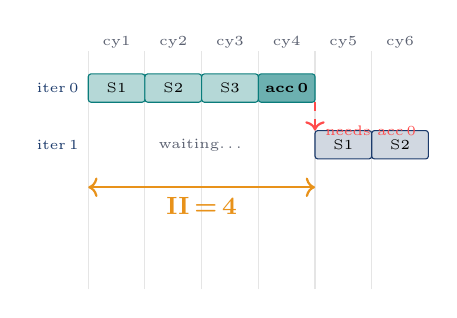
\begin{tikzpicture}[scale=0.72,font=\footnotesize]
    % cycle columns
    \foreach \x in {0,...,5}
      \draw[gray!20,thin] (\x,0)--(\x,4.2);
    \foreach \x/\l in {0/cy1,1/cy2,2/cy3,3/cy4,4/cy5,5/cy6}
      \node[font=\tiny\color{MidGray}] at (\x+0.5,4.35) {\l};

    % iter 0 pipeline stages
    \filldraw[fill=Teal!30,draw=Teal,rounded corners=1pt]
      (0,3.3) rectangle (1,3.8) node[midway,font=\tiny]{S1};
    \filldraw[fill=Teal!30,draw=Teal,rounded corners=1pt]
      (1,3.3) rectangle (2,3.8) node[midway,font=\tiny]{S2};
    \filldraw[fill=Teal!30,draw=Teal,rounded corners=1pt]
      (2,3.3) rectangle (3,3.8) node[midway,font=\tiny]{S3};
    \filldraw[fill=Teal!60,draw=Teal,rounded corners=1pt]
      (3,3.3) rectangle (4,3.8) node[midway,font=\tiny\bfseries]{acc\,0};
    \node[left,font=\tiny\color{Navy}] at (0,3.55) {iter\,0};

    % iter 1 can only start at cy5 (after acc0 ready at cy4)
    \filldraw[fill=Navy!20,draw=Navy,rounded corners=1pt]
      (4,2.3) rectangle (5,2.8) node[midway,font=\tiny]{S1};
    \filldraw[fill=Navy!20,draw=Navy,rounded corners=1pt]
      (5,2.3) rectangle (6,2.8) node[midway,font=\tiny]{S2};
    \node[left,font=\tiny\color{Navy}] at (0,2.55) {iter\,1};
    \node[font=\tiny\color{MidGray}] at (2,2.55) {waiting\ldots};

    % II brace
    \draw[<->,thick,Orange] (0,1.8)--(4,1.8)
      node[midway,below,font=\small\color{Orange}]{\textbf{II\,=\,4}};

    % dependency arrow
    \draw[->,dashed,red!70,thick] (4,3.3)--(4,2.8)
      node[right,font=\tiny\color{red!70}]{needs acc\,0};
  \end{tikzpicture}

  \column{0.48\textwidth}
  \vspace{0.2cm}

  \colorbox{Orange!10}{\parbox{\dimexpr\linewidth-2\fboxsep\relax}{\vspace{4pt}
    {\color{Orange}\bfseries The dependency chain:}\\[3pt]
    {\small \texttt{acc\,+=\,x} reads \texttt{acc} and writes
    a new \texttt{acc}.\\[2pt]
    The new value is ready after 4 cycles.\\[2pt]
    The next iteration needs that value\\
    $\Rightarrow$ must wait 4 cycles $\Rightarrow$ II\,=\,4.}
  \vspace{4pt}}}

  \vspace{8pt}
  \colorbox{Teal!10}{\parbox{\dimexpr\linewidth-2\fboxsep\relax}{\vspace{4pt}
    {\color{Teal}\bfseries Fix: use \texttt{ap\_fixed}.}\\[2pt]
    {\small A fixed-point adder has \textbf{1-cycle latency}.\\
    Dependency resolves in 1 cycle $\Rightarrow$ II\,=\,1.}
  \vspace{4pt}}}

\end{columns}
\end{frame}

%% ── SLIDE 31 : Introducing ap_fixed ─────────────────────────
\begin{frame}[fragile]{Introducing \texttt{ap\_fixed<W,I>}}
\vspace{0.05cm}
\begin{columns}[T,totalwidth=\textwidth]

  \column{0.48\textwidth}
  {\small\color{Navy}\bfseries Syntax:}
  \vspace{2pt}
\begin{lstlisting}
#include "ap_fixed.h"

// W = total bits, I = integer bits
ap_fixed<16, 8> x;
// 8 integer bits, 8 fractional bits
// range: -128 to +127.996
// resolution: 1/256
\end{lstlisting}

  \vspace{6pt}
  \colorbox{Navy!8}{\parbox{\dimexpr\linewidth-2\fboxsep\relax}{\vspace{3pt}
    {\small Vitis HLS includes \texttt{ap\_fixed.h}.\\
    Works in simulation and synthesis.\\
    Drops in as a replacement for \texttt{float}.}
  \vspace{3pt}}}

  \column{0.50\textwidth}
  \vspace{0.1cm}

  {\small\color{Navy}\bfseries Bit layout for \texttt{ap\_fixed<16,8>}:}
  \vspace{4pt}

  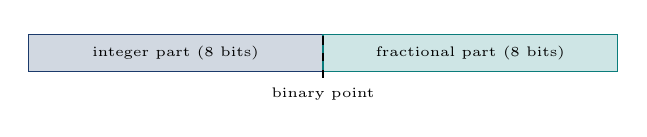
\begin{tikzpicture}[scale=0.78,font=\footnotesize]
    \filldraw[fill=Navy!20,draw=Navy] (0,0) rectangle (4.8,0.6);
    \node at (2.4,0.3) {\tiny integer part (8 bits)};
    \filldraw[fill=Teal!20,draw=Teal] (4.8,0) rectangle (9.6,0.6);
    \node at (7.2,0.3) {\tiny fractional part (8 bits)};
    \draw[dashed,thick] (4.8,-0.1)--(4.8,0.7);
    \node[below,font=\tiny] at (4.8,-0.1) {binary point};
  \end{tikzpicture}

  \vspace{8pt}
  \colorbox{Orange!10}{\parbox{\dimexpr\linewidth-2\fboxsep\relax}{\vspace{3pt}
    {\color{Orange}\bfseries Common rounding modes:}\\[2pt]
    {\small \texttt{AP\_RND} — round to nearest\\
    \texttt{AP\_TRN} — truncate (default, cheapest)\\
    \texttt{AP\_SAT} — saturate on overflow}
  \vspace{3pt}}}

\end{columns}
\end{frame}

%% ── SLIDE 32 : Fixed-point accumulator gives II=1 ────────────
\begin{frame}[fragile]{Fixed-Point Accumulator: II\,=\,1}
\vspace{0.05cm}
\begin{columns}[T,totalwidth=\textwidth]

  \column{0.46\textwidth}
  {\small\color{Navy}\bfseries Change one type:}
  \vspace{2pt}
\begin{lstlisting}
// Before: float
float acc = 0;
for(int k=0; k<N; k++){
  #pragma HLS PIPELINE II=1
  acc += A[i][k]*B[k][j];
}

// After: ap_fixed
ap_fixed<32,16> acc = 0;
for(int k=0; k<N; k++){
  #pragma HLS PIPELINE II=1
  acc += A[i][k]*B[k][j];
}
\end{lstlisting}

  \column{0.52\textwidth}
  \vspace{0.1cm}

  {\small\color{Navy}\bfseries Synthesis report:}
  \vspace{4pt}

  \begin{tabular}{lll}
    \hline
    \rowcolor{Navy!10} & \textbf{float} & \textbf{ap\_fixed}\\
    \hline
    II achieved  & \textbf{\color{Orange}4} & \textbf{\color{GreenHi}1}\\
    \rowcolor{Navy!5}LUT          & 1842 & 312\\
    DSP          & 9    & 6\\
    \rowcolor{Navy!5}Latency (cy) & 257  & 66\\
    \hline
  \end{tabular}

  \vspace{8pt}
  \colorbox{Teal!10}{\parbox{\dimexpr\linewidth-2\fboxsep\relax}{\vspace{3pt}
    {\color{Teal}\bfseries $4\times$ faster, $6\times$ fewer LUTs.}\\[2pt]
    {\small The only change was the type of \texttt{acc}.
    HLS infers a 1-cycle adder automatically.}
  \vspace{3pt}}}

\end{columns}
\end{frame}

%% ── SLIDE 33 : Choosing W and I ──────────────────────────────
\begin{frame}{Choosing W and I}
\vspace{0.1cm}
\begin{columns}[T,totalwidth=\textwidth]

  \column{0.49\textwidth}

  \colorbox{Navy!8}{\parbox{\dimexpr\linewidth-2\fboxsep\relax}{\vspace{3pt}
    {\color{Navy}\bfseries I — integer bits (range):}\\[2pt]
    {\small Enough to hold the max value without overflow.\\[1pt]
    $I \geq \lceil\log_2(\text{max})\rceil + 1$\,(sign).\\[1pt]
    E.g.\ max $= 64 \Rightarrow I = \lceil\log_2(64)\rceil + 1 = 7$.}
  \vspace{3pt}}}

  \vspace{6pt}
  \colorbox{Teal!10}{\parbox{\dimexpr\linewidth-2\fboxsep\relax}{\vspace{3pt}
    {\color{Teal}\bfseries W$-$I — fractional bits (precision):}\\[2pt]
    {\small More bits = lower quantisation error.\\[1pt]
    Pick smallest W that meets your accuracy spec.\\[1pt]
    Start with \texttt{ap\_fixed<16,8>}.}
  \vspace{3pt}}}

  \column{0.02\textwidth}

  \column{0.49\textwidth}
  \vspace{0.1cm}

  {\small\color{Navy}\bfseries Area scales with W:}
  \vspace{4pt}

  \begin{tabular}{lp{0.9cm}p{0.6cm}}
    \hline
    \rowcolor{Navy!10}\textbf{Type} & \textbf{LUT} & \textbf{II}\\
    \hline
    \texttt{ap\_fixed<8,4>}   & $\sim$8   & 1\\
    \rowcolor{Navy!5}\texttt{ap\_fixed<16,8>}  & $\sim$16  & 1\\
    \texttt{ap\_fixed<32,16>} & $\sim$32  & 1\\
    \rowcolor{Navy!5}\texttt{float} (32-bit)   & $\sim$400 & 4\\
    \hline
  \end{tabular}

  \vspace{8pt}
  {\small\color{Orange}\bfseries Workflow:} {\small simulate with float
  first, measure the dynamic range, then pick W and I.}

\end{columns}
\end{frame}

%% ── SLIDE 34 : Accuracy and Quantisation ─────────────────────
\begin{frame}{Accuracy \& Quantisation}
\vspace{0.1cm}
\begin{columns}[T,totalwidth=\textwidth]

  \column{0.49\textwidth}

  {\small Reducing W introduces \textbf{quantisation error}:}
  \vspace{4pt}

  \colorbox{Orange!10}{\parbox{\dimexpr\linewidth-2\fboxsep\relax}{\vspace{3pt}
    {\color{Orange}\bfseries Quantisation step} $= 2^{-(W-I)}$\\[2pt]
    {\small For \texttt{ap\_fixed<16,8>}: step $= 2^{-8} \approx 0.004$.\\
    Values are rounded to the nearest multiple.}
  \vspace{3pt}}}

  \vspace{8pt}
  {\small\color{Navy}\bfseries When accuracy matters:}
  \begin{itemize}\setlength{\itemsep}{1pt}
    {\small
    \item Neural network weights: 8-bit often fine
    \item DSP filters: 16--18 bits typical
    \item Scientific computing: float or double}
  \end{itemize}

  \column{0.02\textwidth}

  \column{0.49\textwidth}
  \vspace{0.1cm}

  \colorbox{Teal!10}{\parbox{\dimexpr\linewidth-2\fboxsep\relax}{\vspace{4pt}
    {\color{Teal}\bfseries Verification approach:}\\[3pt]
    {\small
    1.\ Run C simulation with \texttt{float} (golden reference).\\[2pt]
    2.\ Switch to \texttt{ap\_fixed} and re-simulate.\\[2pt]
    3.\ Compare outputs — measure MSE or max error.\\[2pt]
    4.\ Increase W if accuracy insufficient.\\[2pt]
    5.\ HLS co-simulation confirms HW matches SW.}
  \vspace{4pt}}}

  \vspace{8pt}
  {\small\color{MidGray}\itshape Vitis HLS runs the same C++ test bench
  for both software and RTL simulation.}

\end{columns}
\end{frame}

%% ── SLIDE 35 : Code: float to ap_fixed ───────────────────────
\begin{frame}[fragile]{Code: Replacing \texttt{float} with \texttt{ap\_fixed}}
\vspace{0.05cm}
\begin{columns}[T,totalwidth=\textwidth]

  \column{0.50\textwidth}
  {\small\color{Navy}\bfseries Before (float):}
  \vspace{2pt}
\begin{lstlisting}
void gemm(float A[][N],
          float B[][N],
          float C[][N]){
 for(int i=0;i<N;i++)
  for(int j=0;j<N;j++){
   float acc=0.0f;
   for(int k=0;k<N;k++){
    #pragma HLS PIPELINE
    acc+=A[i][k]*B[k][j];
   }
   C[i][j]=acc;
  }
}
\end{lstlisting}

  \column{0.48\textwidth}
  {\small\color{Navy}\bfseries After (ap\_fixed):}
  \vspace{2pt}
\begin{lstlisting}
#include "ap_fixed.h"
typedef ap_fixed<16,8> fx_t;

void gemm(fx_t A[][N],
          fx_t B[][N],
          fx_t C[][N]){
 for(int i=0;i<N;i++)
  for(int j=0;j<N;j++){
   fx_t acc=0;
   for(int k=0;k<N;k++){
    #pragma HLS PIPELINE
    acc+=A[i][k]*B[k][j];
   }
   C[i][j]=acc;
  }
}
\end{lstlisting}

\end{columns}
\end{frame}

%% ── SLIDE 36 : Full comparison table ────────────────────────
\begin{frame}{Float vs.\ Fixed: Full Comparison}
\vspace{0.15cm}
\begin{columns}[T,totalwidth=\textwidth]

  \column{0.56\textwidth}

  \begin{tabular}{p{2.4cm}p{1.5cm}p{1.8cm}}
    \hline
    \rowcolor{Navy!10}\textbf{Property} & \textbf{float} & \textbf{ap\_fixed<16,8>}\\
    \hline
    Adder latency   & 4 cy        & 1 cy\\
    \rowcolor{Navy!5}Adder LUT       & $\sim$400   & $\sim$16\\
    Mul latency     & 3 cy        & 1--2 cy\\
    \rowcolor{Navy!5}Mul DSP         & 3           & 1\\
    Range           & $\pm 10^{38}$ & $\pm128$\\
    \rowcolor{Navy!5}Precision       & 24-bit M    & 8 frac.\ bits\\
    II (accum.)     & 4           & 1\\
    \rowcolor{Navy!5}Code change     & none        & typedef\\
    \hline
  \end{tabular}

  \column{0.42\textwidth}
  \vspace{0.2cm}

  \colorbox{Orange!10}{\parbox{\dimexpr\linewidth-2\fboxsep\relax}{\vspace{4pt}
    {\color{Orange}\bfseries Use float when:}\\[2pt]
    {\small Wide dynamic range needed\\
    Accuracy is critical\\
    Area/speed not the bottleneck}
  \vspace{4pt}}}

  \vspace{8pt}
  \colorbox{Teal!10}{\parbox{\dimexpr\linewidth-2\fboxsep\relax}{\vspace{4pt}
    {\color{Teal}\bfseries Use ap\_fixed when:}\\[2pt]
    {\small Targeting II\,=\,1 on accumulation\\
    Area budget is tight\\
    Input range is bounded \& known}
  \vspace{4pt}}}

\end{columns}
\end{frame}

%% ── SLIDE 37 : Section 6 takeaways ──────────────────────────
\begin{frame}{Float vs.\ Fixed --- Key Takeaways}
\vspace{0.15cm}
\begin{columns}[T,totalwidth=\textwidth]
  \column{0.50\textwidth}

  \colorbox{Navy!8}{\parbox{\dimexpr\linewidth-2\fboxsep\relax}{\vspace{4pt}
    \textbf{\color{Navy}1.\ Float is a pipeline, not a gate}\\[2pt]
    {\small A float adder has 4 stages. That latency
    propagates directly into II for any loop-carried sum.}
  \vspace{4pt}}}
  \vspace{6pt}

  \colorbox{Teal!10}{\parbox{\dimexpr\linewidth-2\fboxsep\relax}{\vspace{4pt}
    \textbf{\color{Teal}2.\ ap\_fixed breaks the dependency}\\[2pt]
    {\small 1-cycle adder $\Rightarrow$ II\,=\,1.
    Same pragma, same loop, one typedef change.}
  \vspace{4pt}}}
  \vspace{6pt}

  \colorbox{Orange!10}{\parbox{\dimexpr\linewidth-2\fboxsep\relax}{\vspace{4pt}
    \textbf{\color{Orange}3.\ Choose W and I from data, not habit}\\[2pt]
    {\small Simulate in float, measure range, pick W.}
  \vspace{4pt}}}

  \column{0.48\textwidth}
  \vspace{0.2cm}

  \begin{tabular}{lcc}
    \hline
    \rowcolor{Navy!10} & \textbf{float} & \textbf{ap\_fixed}\\
    \hline
    II      & 4 & \textbf{\color{GreenHi}1}\\
    \rowcolor{Navy!5}LUT     & 1842 & \textbf{\color{GreenHi}312}\\
    Latency & 257 cy & \textbf{\color{GreenHi}66 cy}\\
    \hline
  \end{tabular}

  \vspace{10pt}
  {\small\color{MidGray}\itshape These numbers are for the GEMM inner
  loop, $N=64$, on Zynq-7020 @ 100\,MHz.
  Your lab results should be close.}

\end{columns}
\end{frame}

%% ════════════════════════════════════════════════════════════
%%  SECTION 7 --- Summary
%% ════════════════════════════════════════════════════════════

%% ── SLIDE 38 : L6 Key Takeaways ─────────────────────────────
\begin{frame}{L6 Key Takeaways}
\vspace{0.05cm}
\begin{columns}[T,totalwidth=\textwidth]
  \column{0.50\textwidth}

  \colorbox{Navy!8}{\parbox{\dimexpr\linewidth-2\fboxsep\relax}{\vspace{2pt}
    \textbf{\color{Navy}II determines throughput}\\[0pt]
    {\small Throughput $= 1/(\text{II} \times T_\text{clk})$. Minimise II first.}
  \vspace{2pt}}}
  \vspace{3pt}

  \colorbox{Teal!10}{\parbox{\dimexpr\linewidth-2\fboxsep\relax}{\vspace{2pt}
    \textbf{\color{Teal}Pragma order matters}\\[0pt]
    {\small PIPELINE $\to$ ARRAY\_PARTITION $\to$ UNROLL.}
  \vspace{2pt}}}
  \vspace{3pt}

  \colorbox{Orange!10}{\parbox{\dimexpr\linewidth-2\fboxsep\relax}{\vspace{2pt}
    \textbf{\color{Orange}Float costs area and II}\\[0pt]
    {\small \texttt{ap\_fixed} recovers II\,=\,1, cuts LUT count.}
  \vspace{2pt}}}
  \vspace{3pt}

  \colorbox{Navy!8}{\parbox{\dimexpr\linewidth-2\fboxsep\relax}{\vspace{2pt}
    \textbf{\color{Navy}Read the report}\\[0pt]
    {\small Let numbers drive every pragma decision.}
  \vspace{2pt}}}

  \column{0.48\textwidth}
  \vspace{0.2cm}

  \begin{tabular}{lcc}
    \hline
    \rowcolor{Navy!10}\textbf{Version} & \textbf{II} & \textbf{Speedup}\\
    \hline
    Baseline                       & 7 & $1\times$\\
    \rowcolor{Navy!5}+ PIPELINE (float) & 4 & ${\approx}1.7\times$\\
    + ap\_fixed + PIPELINE         & 1 & $7\times$\\
    \rowcolor{Navy!5}+ UNROLL$\times$4  & 1 & ${\approx}28\times$\\
    \hline
  \end{tabular}

  \vspace{10pt}
  {\small\color{MidGray}\itshape The final design is ${\approx}28\times$ faster
  than baseline with lower LUT count than the float pipeline version.}

\end{columns}
\end{frame}

%% ── SLIDE 39 : What's Next ───────────────────────────────────
\begin{frame}{What's Next --- L7 Preview}
\vspace{0.2cm}
\begin{columns}[T,totalwidth=\textwidth]
  \column{0.52\textwidth}

  \colorbox{Navy!8}{\parbox{\dimexpr\linewidth-2\fboxsep\relax}{\vspace{5pt}
    \textbf{L7 --- Quantisation \& Accuracy}\\[5pt]
    \hspace{6pt}$\bullet$\ Measuring quantisation error\\[2pt]
    \hspace{6pt}$\bullet$\ Fixed-point simulation in C++\\[2pt]
    \hspace{6pt}$\bullet$\ Word-length optimisation methodology\\[2pt]
    \hspace{6pt}$\bullet$\ Case study: FIR filter in \texttt{ap\_fixed}
  \vspace{5pt}}}

  \vspace{10pt}
  {\small\color{MidGray}\itshape Before L7: complete the lab --- apply
  the pragmas, record synthesis reports, note where II changes.}

  \column{0.46\textwidth}
  \vspace{0.3cm}

  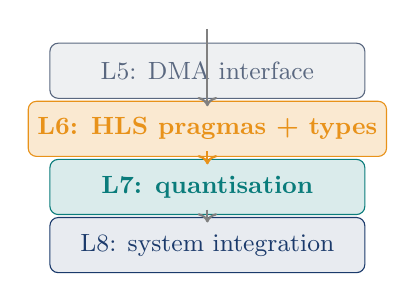
\begin{tikzpicture}[scale=0.82,font=\small]
    \node[draw=BoxGray,fill=BoxGray!10,rounded corners=3pt,
          minimum width=4.0cm,minimum height=0.7cm,align=center]
      at (0,3.2) {\color{BoxGray} L5: DMA interface};
    \node[draw=Orange,fill=Orange!20,rounded corners=3pt,
          minimum width=4.0cm,minimum height=0.7cm,align=center]
      at (0,2.3) {\color{Orange}\bfseries L6: HLS pragmas + types};
    \node[draw=Teal,fill=Teal!15,rounded corners=3pt,
          minimum width=4.0cm,minimum height=0.7cm,align=center]
      at (0,1.4) {\color{Teal}\bfseries L7: quantisation};
    \node[draw=Navy,fill=Navy!10,rounded corners=3pt,
          minimum width=4.0cm,minimum height=0.7cm,align=center]
      at (0,0.5) {\color{Navy} L8: system integration};
    \draw[->,thick,Orange] (0,1.95)--(0,1.75);
    \draw[->,thick,gray]   (0,3.85)--(0,2.65);
    \draw[->,thick,gray]   (0,1.05)--(0,0.85);
  \end{tikzpicture}
\end{columns}
\end{frame}

%% ── SLIDE 40 : Questions ─────────────────────────────────────
{
\setbeamercolor{background canvas}{bg=NavyDk}
\setbeamertemplate{footline}{%
  \vspace{2pt}%
  \hspace{0.6cm}{\color{LtGray}\fontsize{7.5}{9}\selectfont
    Hardware / Software Codesign \enspace|\enspace 2025/26 \enspace|\enspace IST}%
  \hfill%
  {\color{LtGray}\fontsize{7.5}{9}\selectfont\insertframenumber}%
  \hspace{0.5cm}\vspace{3pt}%
}
\begin{frame}[plain]
  \vspace{1.5cm}
  \begin{center}
    {\color{white}\fontsize{36}{42}\selectfont\textbf{Questions?}}\\[0.6cm]
    {\color{LtGray}\fontsize{13}{16}\selectfont
      L6 \enspace$\cdot$\enspace HLS Optimisation \& Float/Fixed Intro}\\[0.3cm]
    {\color{LtGray}\fontsize{10}{12}\selectfont
      José T.\ de Sousa \enspace$\cdot$\enspace IST \enspace$\cdot$\enspace 2025/26}
  \end{center}
  \vspace{0.8cm}
  \begin{center}
  
\begin{tikzpicture}[
    box/.style={rounded corners=3pt, minimum width=2.6cm, minimum height=0.9cm,
                align=center, font=\small\bfseries},
    node distance=0.35cm
  ]
    \node[box, fill=BoxGray!80, text=white] (ip)  {II\,=\,1};
    \node[box, fill=Orange,     text=white, right=of ip]  (pp) {PIPELINE};
    \node[box, fill=Navy,       text=white, right=of pp]  (fl) {ap\_fixed};
    \node[box, fill=Teal,       text=white, right=of fl]  (fx) {read report};
  \end{tikzpicture}
  \end{center}
\end{frame}
}

\end{document}
    \node[box, fill=Navy,       text=white, right=of pp]